\documentclass{beamer}
\usepackage[utf8]{inputenc}

\usetheme{Madrid}
\usecolortheme{default}
\usepackage{amsmath,amssymb,amsfonts,amsthm}
\usepackage{txfonts}
\usepackage{tkz-euclide}
\usepackage{listings}
\usepackage{adjustbox}
\usepackage{array}
\usepackage{tabularx}
\usepackage{gvv}
\usepackage{lmodern}
\usepackage{circuitikz}
\usepackage{tikz}
\usepackage{graphicx}

\setbeamertemplate{page number in head/foot}[totalframenumber]

\usepackage{tcolorbox}
\tcbuselibrary{minted,breakable,xparse,skins}



\definecolor{bg}{gray}{0.95}
\DeclareTCBListing{mintedbox}{O{}m!O{}}{%
	breakable=true,
	listing engine=minted,
	listing only,
	minted language=#2,
	minted style=default,
	minted options={%
		linenos,
		gobble=0,
		breaklines=true,
		breakafter=,,
		fontsize=\small,
		numbersep=8pt,
		#1},
	boxsep=0pt,
	left skip=0pt,
	right skip=0pt,
	left=25pt,
	right=0pt,
	top=3pt,
	bottom=3pt,
	arc=5pt,
	leftrule=0pt,
	rightrule=0pt,
	bottomrule=2pt,
	toprule=2pt,
	colback=bg,
	colframe=orange!70,
	enhanced,
	overlay={%
		\begin{tcbclipinterior}
			\fill[orange!20!white] (frame.south west) rectangle ([xshift=20pt]frame.north west);
	\end{tcbclipinterior}},
	#3,
}
\lstset{
	language=C,
	basicstyle=\ttfamily\small,
	keywordstyle=\color{blue},
	stringstyle=\color{orange},
	commentstyle=\color{green!60!black},
	numbers=left,
	numberstyle=\tiny\color{gray},
	breaklines=true,
	showstringspaces=false,
}
\begin{document}

\title 
{2.4.37}
\date{6 September,2025}

\author 
{Naman Kumar-EE25BTECH11041}
\graphicspath{./figs}


\frame{\titlepage}
\begin{frame}{Question}
If a variable line in two adjacent positions has directions cosines l, m, n and $l+\delta l, m+\delta m, n +\delta n$, show that the small angle $\delta\theta$ between the two positions is given by
\begin{center}
    $\delta\theta^2=(\delta l)^2+(\delta m)^2+(\delta n)^2$
\end{center}
\end{frame}
\begin{frame}{Solution}
    We know about direction cosine of any vector,
\begin{align}
    l^2+m^2+n^2=1 \label{1}
\end{align}
and angle between two vectors
\begin{align}
    \cos{\theta}=\frac{\Vec{A}^T\Vec{B}}{\lVert\Vec{A}\rVert\lVert\Vec{B}\rVert} \label{2}
\end{align}
We also know expansion of $\cos{\delta x}$ ($\delta x$ represents very small x)
\begin{align}
    \cos{x}= 1-\frac{x^2}{2!}+\frac{x^4}{4!}.... \label{3}
\end{align}
Given Two direction cosine
\begin{align}
    l,m,n \text{ and } l+\delta l,m+\delta m,n+\delta n
\end{align}
\end{frame}
\begin{frame}{Solution}
Using $\eqref{1}$ for both direction cosines
\begin{align}
    l^2+m^2+n^2=1
\end{align}
and
\begin{align}
    (l+\delta l)^2+(m+\delta m)^2+(n+\delta n)^2=1\\
    l^2+m^2+n^2+(\delta l)^2+(\delta m)^2+(\delta n)^2+2(l\delta l+m\delta m+n\delta n)=1
\end{align}
from $\eqref{1}$
\begin{align}
    1+(\delta l)^2+(\delta m)^2+(\delta n)^2+2(l\delta l+m\delta m+n\delta n)=1\\
    (\delta l)^2+(\delta m)^2+(\delta n)^2=-2(l\delta l+m\delta m+n\delta n) \label{9}
\end{align}
\end{frame}
\begin{frame}{Solution}
Using equation $\eqref{2}$
\begin{align}
    \cos{\theta}=\frac{\begin{pmatrix}l\\m\\n\end{pmatrix}^T \begin{pmatrix}l+\delta l\\m+\delta m\\n+\delta n\end{pmatrix}^T}{1\times 1}\\
    \cos{\theta}=l(l+\delta l)+m(m+\delta m)+n(n+\delta n)\\
    \cos{\theta}=l^2+m^2+n^2+l\delta l+m\delta m+n\delta n\\
\end{align}
using equation $\eqref{1}$ $\eqref{3}$ and $\eqref{9}$
\begin{align}
    1-\frac{\delta\theta^2}{2!}=1+\frac{1}{-2}(\delta l)^2+(\delta m)^2+(\delta n)^2
\end{align}
Where $\delta\theta$ represents very small $\theta$
\begin{align}
    \delta\theta^2=(\delta l)^2+(\delta m)^2+(\delta n)^2
\end{align}
Hence Proved
\end{frame}
\begin{frame}{Figure}
    \begin{figure}[H]
    \centering
    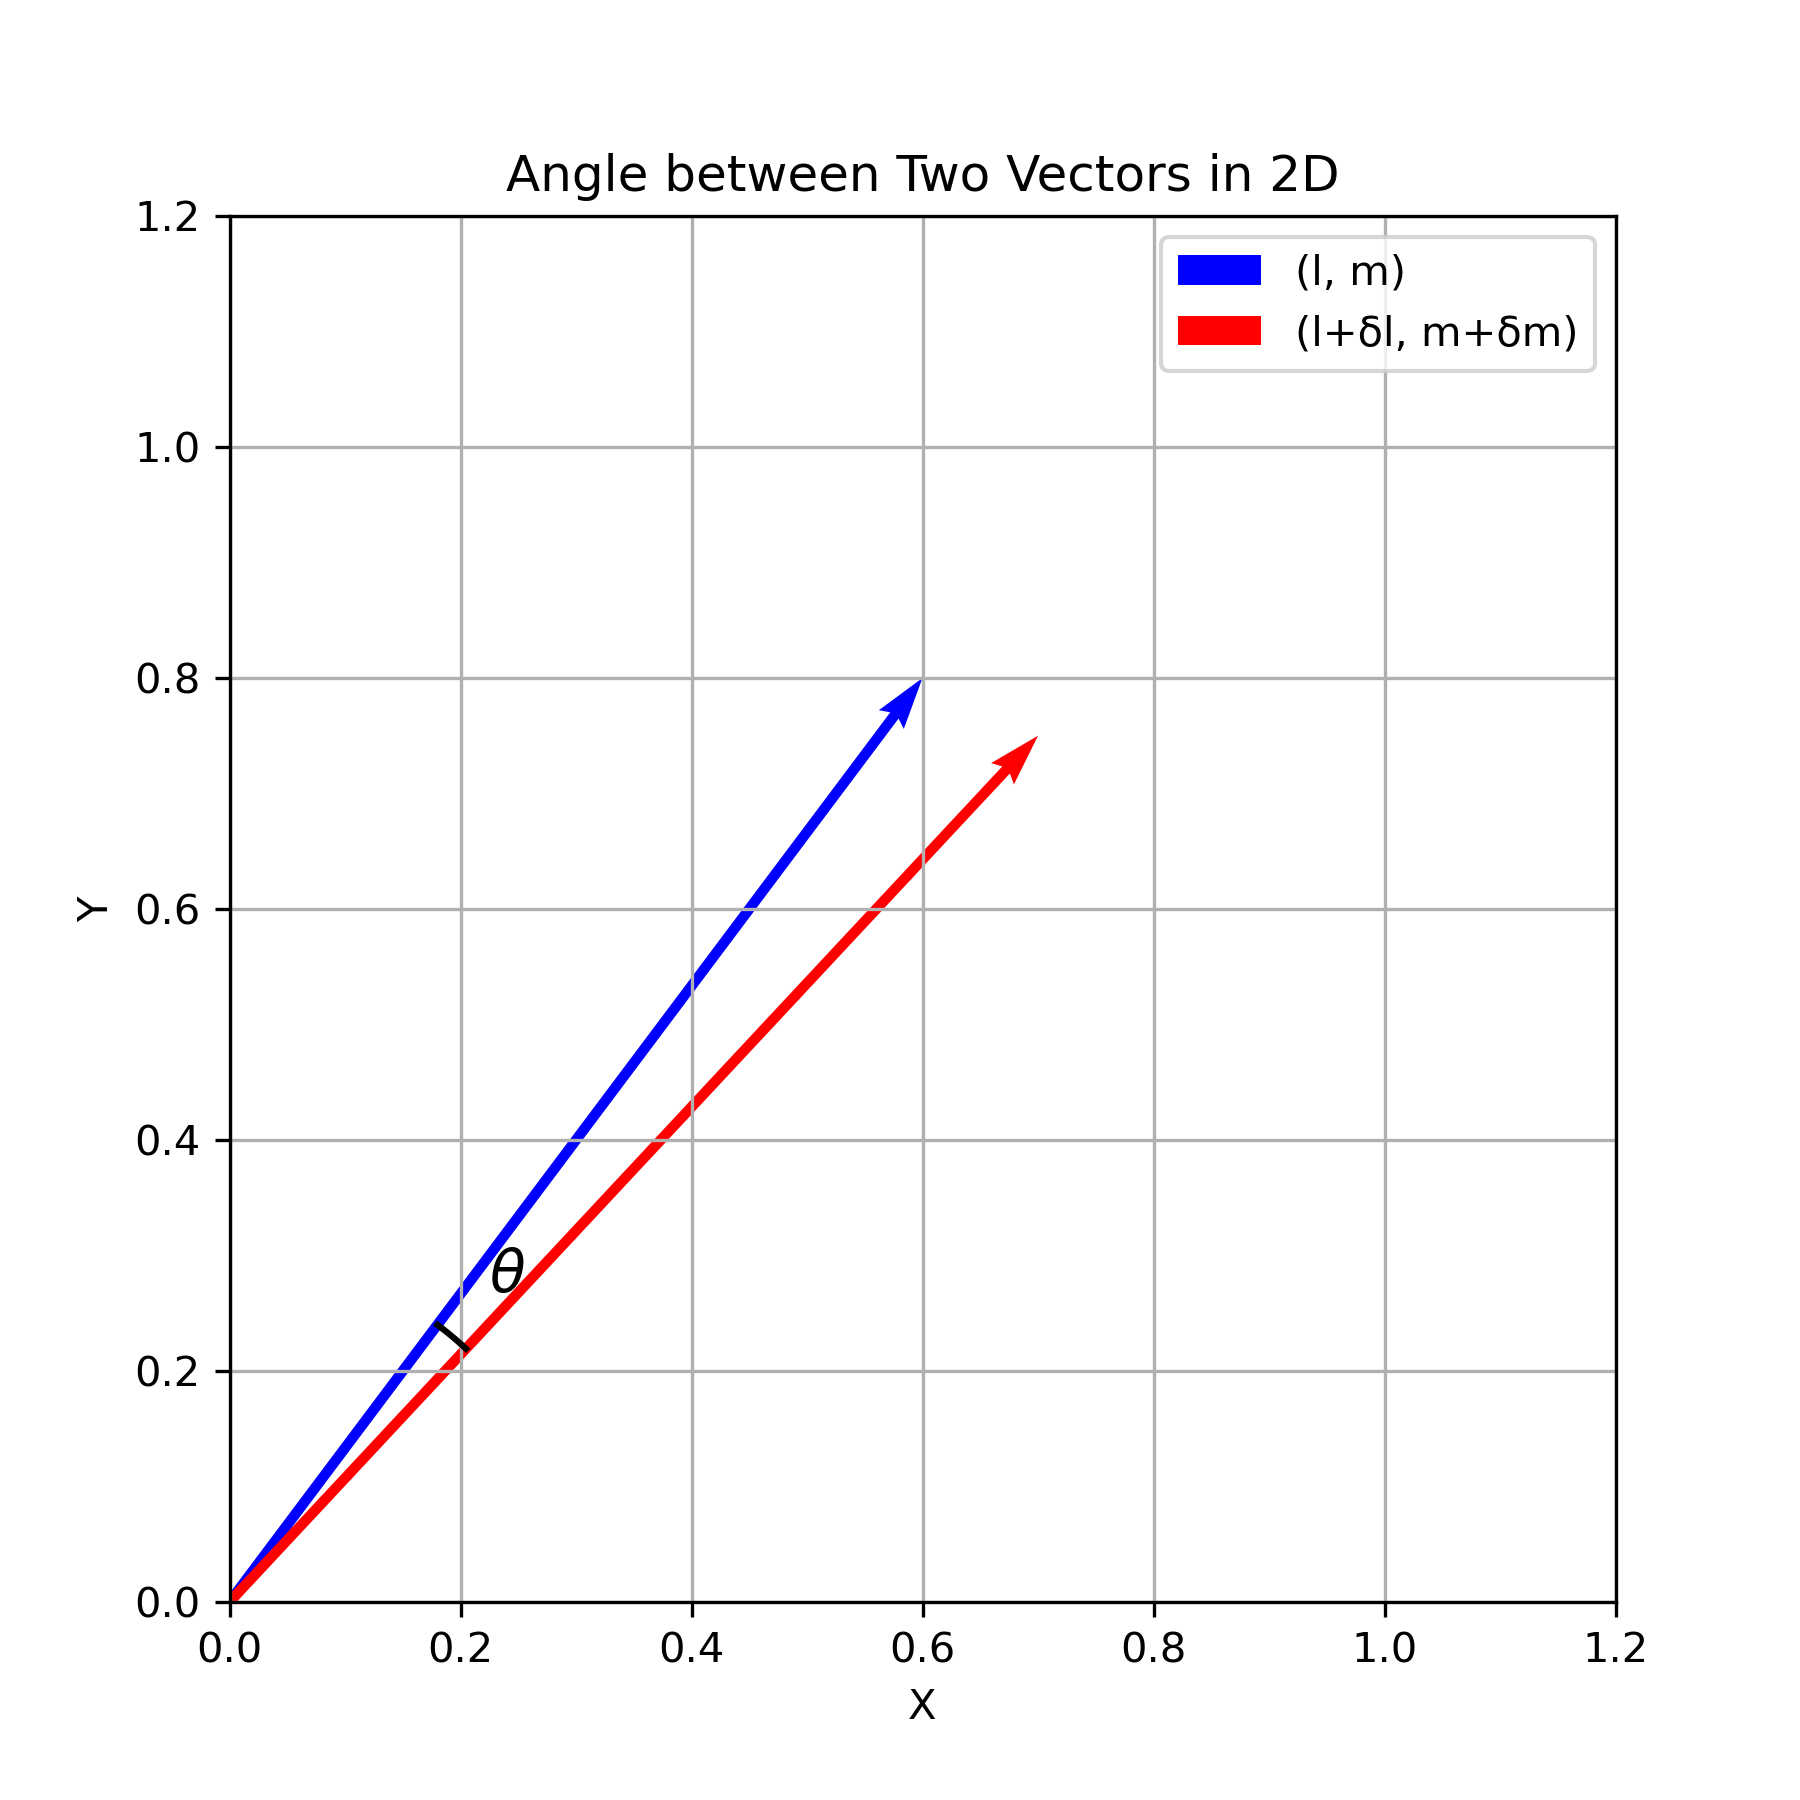
\includegraphics[width=0.6\columnwidth]{figs/vectors.png}
    \caption{Caption}
    \label{fig:placeholder}
\end{figure}
\end{frame}

\begin{frame}[fragile]
\frametitle{C code}
\begin{lstlisting}
#include <stdio.h>
#include <math.h>
void dot_product(double v1[], double v2[], int size, double* result) {
    *result = 0.0;
    for (int i = 0; i < size; i++) {
        *result += v1[i] * v2[i];
    }
    return result;
}
\end{lstlisting}
\end{frame}
\begin{frame}[fragile]
\frametitle{Python from Shared Object}
\begin{lstlisting}
import numpy as np
import matplotlib.pyplot as plt
import ctypes

# Load the shared library
lib = ctypes.CDLL("./libdot.so")

# Define function signature
lib.dot_product.argtypes = [
    np.ctypeslib.ndpointer(dtype=np.double),
    np.ctypeslib.ndpointer(dtype=np.double),
    ctypes.c_int,
    ctypes.POINTER(ctypes.c_double)
]
\end{lstlisting}
\end{frame}
\begin{frame}[fragile]
\frametitle{Python from Shared Object}
\begin{lstlisting}
# Vectors
l, m = 0.6, 0.8
dl, dm = 0.1, -0.05

v1 = np.array([l, m], dtype=np.double)
v2 = np.array([l+dl, m+dm], dtype=np.double)

# Call C function for dot product
res = ctypes.c_double()
lib.dot_product(v1, v2, 2, ctypes.byref(res))
dot = res.value

# Normalize
v1u = v1 / np.linalg.norm(v1)
v2u = v2 / np.linalg.norm(v2)
\end{lstlisting}
\end{frame}
\begin{frame}[fragile]
\frametitle{Python from Shared Object}
\begin{lstlisting}
# Angle between vectors
theta = np.arccos(np.clip(dot / (np.linalg.norm(v1) * np.linalg.norm(v2)), -1.0, 1.0))

# Angles relative to x-axis
a1 = np.arctan2(v1u[1], v1u[0])
a2 = np.arctan2(v2u[1], v2u[0])
start, end = sorted([a1, a2])

# Plot
fig, ax = plt.subplots(figsize=(6,6))

ax.quiver(0, 0, v1[0], v1[1], angles='xy', scale_units='xy', scale=1, color='b', label='(l,m)')
ax.quiver(0, 0, v2[0], v2[1], angles='xy', scale_units='xy', scale=1, color='r', label='(l+dl,m+dm)')
\end{lstlisting}
\end{frame}
\begin{frame}[fragile]
\frametitle{Python from Shared Object}
\begin{lstlisting}
# Arc for angle
r = 0.3
arc_angles = np.linspace(start, end, 100)
arc_x = r * np.cos(arc_angles)
arc_y = r * np.sin(arc_angles)
ax.plot(arc_x, arc_y, 'k-')

# Label theta
mid = (start + end) / 2
ax.text(0.35*np.cos(mid), 0.35*np.sin(mid), r'$\theta$', fontsize=14)
\end{lstlisting}
\end{frame}
\begin{frame}[fragile]
\frametitle{Python from Shared Object}
\begin{lstlisting}
# Formatting
ax.set_xlim(0, 1.2)
ax.set_ylim(0, 1.2)
ax.set_aspect('equal')
ax.set_xlabel("X")
ax.set_ylabel("Y")
ax.set_title("Angle between two vectors (C + Python)")
ax.legend()
ax.grid(True)

plt.savefig("vectors.png", dpi=300)
plt.show()
\end{lstlisting}
\end{frame}
\begin{frame}[fragile]
\frametitle{Direct Python }
\begin{lstlisting}
import numpy as np
import matplotlib.pyplot as plt

# Example direction cosines (2D projection)
l, m = 0.6, 0.8
dl, dm = 0.1, -0.05

# Vectors
v1 = np.array([l, m])
v2 = np.array([l+dl, m+dm])

# Normalize
v1_u = v1 / np.linalg.norm(v1)
v2_u = v2 / np.linalg.norm(v2)
\end{lstlisting}
\end{frame}
\begin{frame}[fragile]
\frametitle{Direct Python }
\begin{lstlisting}
# Compute their angles w.r.t x-axis
angle1 = np.arctan2(v1_u[1], v1_u[0])
angle2 = np.arctan2(v2_u[1], v2_u[0])

# Ensure correct order (draw smaller arc between them)
start_angle = min(angle1, angle2)
end_angle = max(angle1, angle2)

# Plot
fig, ax = plt.subplots(figsize=(6,6))
\end{lstlisting}
\end{frame}
\begin{frame}[fragile]
\frametitle{Direct Python }
\begin{lstlisting}
# Draw vectors
ax.quiver(0, 0, v1[0], v1[1], angles='xy', scale_units='xy', scale=1, color='b', label='(l, m)')
ax.quiver(0, 0, v2[0], v2[1], angles='xy', scale_units='xy', scale=1, color='r', label='(l+δl, m+δm)')

# Draw arc for angle θ
arc_radius = 0.3
arc_angles = np.linspace(start_angle, end_angle, 100)
arc_x = arc_radius * np.cos(arc_angles)
arc_y = arc_radius * np.sin(arc_angles)
ax.plot(arc_x, arc_y, 'k-')
\end{lstlisting}
\end{frame}
\begin{frame}[fragile]
\frametitle{Direct Python }
\begin{lstlisting}
# Label θ at midpoint of arc
mid_angle = (start_angle + end_angle) / 2
ax.text(0.35*np.cos(mid_angle), 0.35*np.sin(mid_angle), r'$\theta$', fontsize=14)

# Formatting
ax.set_xlim(0, 1.2)
ax.set_ylim(0, 1.2)
ax.set_aspect('equal')
ax.set_xlabel("X")
ax.set_ylabel("Y")
ax.set_title("Angle between Two Vectors in 2D")
ax.legend()
ax.grid(True)

# Save figure
plt.savefig("vectors.png", dpi=300)
plt.show()

\end{lstlisting}
\end{frame}

\end{document}